\DocumentMetadata{
  pdfstandard={a-4f,ua-2},
  tagging=on,
  xmp=true}
% Options for packages loaded elsewhere
% Options for packages loaded elsewhere
\PassOptionsToPackage{unicode}{hyperref}
\PassOptionsToPackage{hyphens}{url}
\PassOptionsToPackage{dvipsnames,svgnames,x11names}{xcolor}
%
\documentclass[
  12pt,
  letterpaper,
  DIV=11,
  numbers=noendperiod]{scrreprt}
\usepackage{xcolor}
\usepackage[margin=1in]{geometry}
\usepackage{amsmath,amssymb}
\setcounter{secnumdepth}{-\maxdimen} % remove section numbering
\usepackage{iftex}
\ifPDFTeX
  \usepackage[T1]{fontenc}
  \usepackage[utf8]{inputenc}
  \usepackage{textcomp} % provide euro and other symbols
\else % if luatex or xetex
  \usepackage{unicode-math} % this also loads fontspec
  \defaultfontfeatures{Scale=MatchLowercase}
  \defaultfontfeatures[\rmfamily]{Ligatures=TeX,Scale=1}
\fi
\usepackage{lmodern}
\ifPDFTeX\else
  % xetex/luatex font selection
\fi
% Use upquote if available, for straight quotes in verbatim environments
\IfFileExists{upquote.sty}{\usepackage{upquote}}{}
\IfFileExists{microtype.sty}{% use microtype if available
  \usepackage[]{microtype}
  \UseMicrotypeSet[protrusion]{basicmath} % disable protrusion for tt fonts
}{}
\makeatletter
\@ifundefined{KOMAClassName}{% if non-KOMA class
  \IfFileExists{parskip.sty}{%
    \usepackage{parskip}
  }{% else
    \setlength{\parindent}{0pt}
    \setlength{\parskip}{6pt plus 2pt minus 1pt}}
}{% if KOMA class
  \KOMAoptions{parskip=half}}
\makeatother
% Make \paragraph and \subparagraph free-standing
\makeatletter
\ifx\paragraph\undefined\else
  \let\oldparagraph\paragraph
  \renewcommand{\paragraph}{
    \@ifstar
      \xxxParagraphStar
      \xxxParagraphNoStar
  }
  \newcommand{\xxxParagraphStar}[1]{\oldparagraph*{#1}\mbox{}}
  \newcommand{\xxxParagraphNoStar}[1]{\oldparagraph{#1}\mbox{}}
\fi
\ifx\subparagraph\undefined\else
  \let\oldsubparagraph\subparagraph
  \renewcommand{\subparagraph}{
    \@ifstar
      \xxxSubParagraphStar
      \xxxSubParagraphNoStar
  }
  \newcommand{\xxxSubParagraphStar}[1]{\oldsubparagraph*{#1}\mbox{}}
  \newcommand{\xxxSubParagraphNoStar}[1]{\oldsubparagraph{#1}\mbox{}}
\fi
\makeatother


\usepackage{longtable,booktabs,array}
\newcounter{none} % for unnumbered tables
\usepackage{calc} % for calculating minipage widths
% Correct order of tables after \paragraph or \subparagraph
\usepackage{etoolbox}
\makeatletter
\patchcmd\longtable{\par}{\if@noskipsec\mbox{}\fi\par}{}{}
\makeatother
% Allow footnotes in longtable head/foot
\IfFileExists{footnotehyper.sty}{\usepackage{footnotehyper}}{\usepackage{footnote}}
\makesavenoteenv{longtable}
\usepackage{graphicx}
\makeatletter
\newsavebox\pandoc@box
\newcommand*\pandocbounded[1]{% scales image to fit in text height/width
  \sbox\pandoc@box{#1}%
  \Gscale@div\@tempa{\textheight}{\dimexpr\ht\pandoc@box+\dp\pandoc@box\relax}%
  \Gscale@div\@tempb{\linewidth}{\wd\pandoc@box}%
  \ifdim\@tempb\p@<\@tempa\p@\let\@tempa\@tempb\fi% select the smaller of both
  \ifdim\@tempa\p@<\p@\scalebox{\@tempa}{\usebox\pandoc@box}%
  \else\usebox{\pandoc@box}%
  \fi%
}
% Set default figure placement to htbp
\def\fps@figure{htbp}
\makeatother





\setlength{\emergencystretch}{3em} % prevent overfull lines

\providecommand{\tightlist}{%
  \setlength{\itemsep}{0pt}\setlength{\parskip}{0pt}}



 


\usepackage{booktabs}
\usepackage{longtable}
\usepackage{array}
\usepackage{multirow}
\usepackage{wrapfig}
\usepackage{float}
\usepackage{colortbl}
\usepackage{pdflscape}
\usepackage{tabu}
\usepackage{threeparttable}
\usepackage{threeparttablex}
\usepackage[normalem]{ulem}
\usepackage{makecell}
\usepackage{xcolor}
\usepackage{caption}
\usepackage{anyfontsize}
\makeatletter
\renewcommand{\chapter}{%
\global\@topnum\z@
\@afterindentfalse
\secdef\@chapter\@schapter
}
\makeatother
\AtBeginDocument{\let\maketitle\relax}
\usepackage{fancyhdr}
\pagestyle{fancy}
\fancyfoot{}
\fancyhead[L]{WIS2323 - The Future of Rain Forests}
\fancyhead[R]{Syllabus, p. \thepage}
\usepackage{datetime2}
\fancyfoot[R]{Updated \today}
\usepackage{parskip}
\usepackage{xcolor}
\definecolor{darkcerulean}{rgb}{0.03, 0.27, 0.49}
\definecolor{darkmidnightblue}{rgb}{0.0, 0.2, 0.4}
\definecolor{customcharcoal}{RGB}{86, 86, 86}
\usepackage{caption}
\captionsetup[table]{labelformat=empty}
\usepackage{float}
\floatplacement{table}{H}
\usepackage{xcolor}
\usepackage{sectsty}
\captionsetup[table]{labelformat=empty}
\usepackage{float}
\floatplacement{table}{H}
\usepackage{titlesec}
% 1. Redefine the chapter layout (required by titlesec for chapters)
\titleformat{\chapter}[display]
  {\sffamily\color{customcharcoal}\LARGE\bfseries\filcenter}
  {\chaptertitlename\ \thechapter}
  {10pt} % Space between "Chapter X" label and the Title Text
  {\LARGE}

% 2. Adjust the margins around the chapter header
% \titlespacing*{\command}{left-margin}{before-sep}{after-sep}
\titlespacing*{\chapter}{1pt}{5pt}{5pt}
\titlespacing*{\section}{0pt}{3.5ex plus 1ex minus .2ex}{1.5ex plus .2ex}
\titlespacing*{\subsection}{0pt}{3.25ex plus 1ex minus .2ex}{1ex plus .1ex}






\usepackage{sectsty}\chapterfont{\centering\color{customcharcoal}}
\usepackage{sectsty}\sectionfont{\color{darkmidnightblue}}
\usepackage{sectsty}\subsectionfont{\color{customcharcoal}}
\usepackage{sectsty}\subsubsectionfont{\raggedright\color{customcharcoal}}
\KOMAoption{captions}{tableheading}
\makeatletter
\@ifpackageloaded{tcolorbox}{}{\usepackage[skins,breakable]{tcolorbox}}
\@ifpackageloaded{fontawesome5}{}{\usepackage{fontawesome5}}
\definecolor{quarto-callout-color}{HTML}{909090}
\definecolor{quarto-callout-note-color}{HTML}{0758E5}
\definecolor{quarto-callout-important-color}{HTML}{CC1914}
\definecolor{quarto-callout-warning-color}{HTML}{EB9113}
\definecolor{quarto-callout-tip-color}{HTML}{00A047}
\definecolor{quarto-callout-caution-color}{HTML}{FC5300}
\definecolor{quarto-callout-color-frame}{HTML}{acacac}
\definecolor{quarto-callout-note-color-frame}{HTML}{4582ec}
\definecolor{quarto-callout-important-color-frame}{HTML}{d9534f}
\definecolor{quarto-callout-warning-color-frame}{HTML}{f0ad4e}
\definecolor{quarto-callout-tip-color-frame}{HTML}{02b875}
\definecolor{quarto-callout-caution-color-frame}{HTML}{fd7e14}
\makeatother
\makeatletter
\@ifpackageloaded{caption}{}{\usepackage{caption}}
\AtBeginDocument{%
\ifdefined\contentsname
  \renewcommand*\contentsname{Table of contents}
\else
  \newcommand\contentsname{Table of contents}
\fi
\ifdefined\listfigurename
  \renewcommand*\listfigurename{List of Figures}
\else
  \newcommand\listfigurename{List of Figures}
\fi
\ifdefined\listtablename
  \renewcommand*\listtablename{List of Tables}
\else
  \newcommand\listtablename{List of Tables}
\fi
\ifdefined\figurename
  \renewcommand*\figurename{Figure}
\else
  \newcommand\figurename{Figure}
\fi
\ifdefined\tablename
  \renewcommand*\tablename{Table}
\else
  \newcommand\tablename{Table}
\fi
}
\@ifpackageloaded{float}{}{\usepackage{float}}
\floatstyle{ruled}
\@ifundefined{c@chapter}{\newfloat{codelisting}{h}{lop}}{\newfloat{codelisting}{h}{lop}[chapter]}
\floatname{codelisting}{Listing}
\newcommand*\listoflistings{\listof{codelisting}{List of Listings}}
\makeatother
\makeatletter
\makeatother
\makeatletter
\@ifpackageloaded{caption}{}{\usepackage{caption}}
\@ifpackageloaded{subcaption}{}{\usepackage{subcaption}}
\makeatother
\usepackage{bookmark}
\IfFileExists{xurl.sty}{\usepackage{xurl}}{} % add URL line breaks if available
\urlstyle{same}
\hypersetup{
  pdftitle={SLOs},
  pdfauthor={Emilio M. Bruna},
  colorlinks=true,
  linkcolor={blue},
  filecolor={Maroon},
  citecolor={Blue},
  urlcolor={blue},
  pdfcreator={LaTeX via pandoc}}


\title{SLOs}
\author{Emilio M. Bruna}
\date{August 10, 2026}
\begin{document}
\maketitle


\pandocbounded{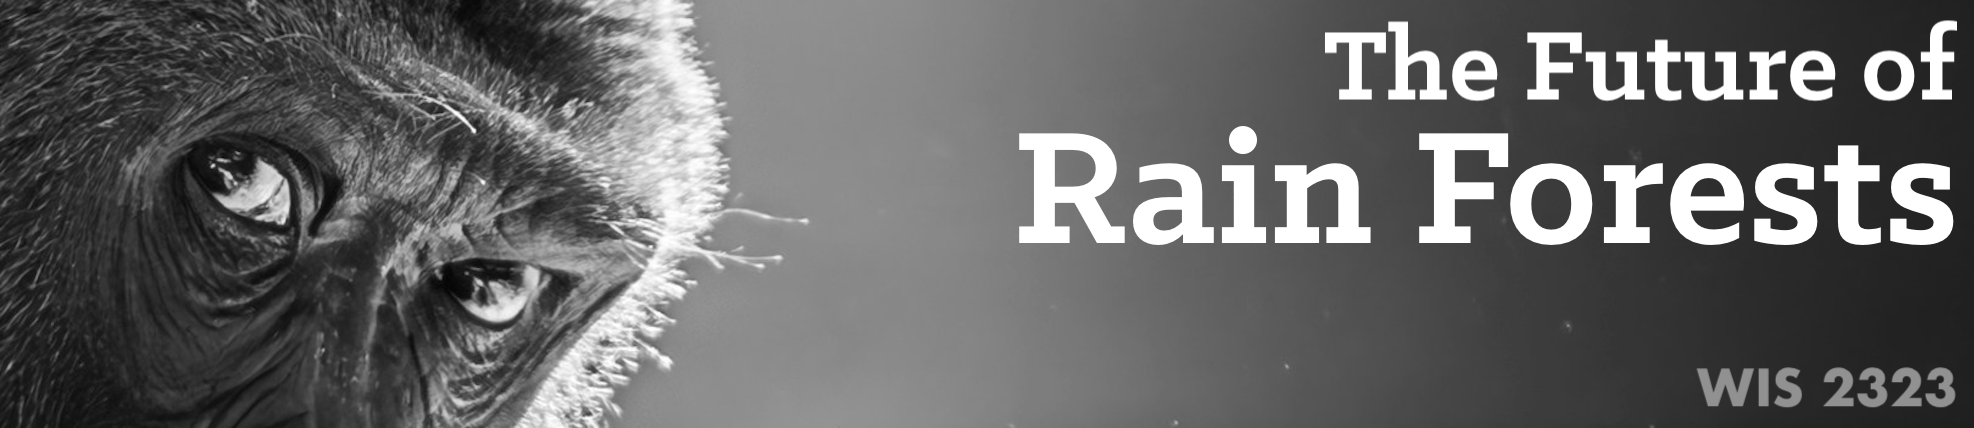
\includegraphics[keepaspectratio]{../images/banner.png}}

\chapter{Syllabus}\label{syllabus}

\section*{Introduction}\label{introduction}
\addcontentsline{toc}{section}{Introduction}

This course investigates the fundamental issues addressed by scientists
studying tropical rain forests, including what gave rise to their
remarkable biodiversity, the drivers and consequences of deforestation,
why people are fascinated by rain forests, cultural and ecological
stereotypes about the tropics, and different approaches to forest
conservation and sustainability. \textbf{\emph{By the end of the course
students will be able to:}}

\begin{itemize}
\tightlist
\item
  Recognize and describe stereotypes about rain forests \& their
  residents
\item
  Analyze rain forest tropes in art, literature, \& popular culture
\item
  Discuss \& evaluate hypotheses for the origins and maintenance of
  tropical biodiversity
\item
  Explain \& compare the history and ecological influence of humans in
  rain forests
\item
  Review contemporary threats to rain forests
\item
  Analyze and visualize data on deforestation
\item
  Review and contrast strategies for rain forest conservation \&
  restoration
\item
  Identify the presence of rain forests in their daily lives \& set
  personal goals for advancing rain forest conservation
\item
  Produce materials for communicating about tropical biology \& the
  conservation of tropical rain forests to family and peers
\end{itemize}

\section*{When \& Where}\label{when-where}
\addcontentsline{toc}{section}{When \& Where}

\textbf{When:} Tuesdays 11:45 AM-12:35 PM \& Thursdays 11:45 AM-1:40
PM\\
\textbf{Where:} Larsen Hall 0310~

\section*{Instructor \& TA}\label{instructor-ta}
\addcontentsline{toc}{section}{Instructor \& TA}

\textbf{Instructor:} Dr.~Emilio M. Bruna,
\href{mailto:embruna@ufl.edu}{\nolinkurl{embruna@ufl.edu}}, (352)
846-0634)~\\
\textbf{Teaching Assistant:} Ashra Kunwar,
\href{mailto:kunwarashra@ufl.edu}{\nolinkurl{kunwarashra@ufl.edu}}

\section*{Credits \& Prerequisites}\label{credits-prerequisites}
\addcontentsline{toc}{section}{Credits \& Prerequisites}

\textbf{Credits:} 3\\
\textbf{Prerequisites:} None\\
\textbf{Quest Designation:} Quest 2\\
\textbf{GenEd Designation:} International

\begin{itemize}
\tightlist
\item
  A minimum grade of C is required for Quest and General Education
  credit.
\item
  Courses intended to satisfy Quest and GenEd requirements \emph{cannot}
  be taken S-U.
\end{itemize}

\section*{Majors, Minors, and
Certificates}\label{majors-minors-and-certificates}
\addcontentsline{toc}{section}{Majors, Minors, and Certificates}

This course counts towards the graduation requirements of the following
UF Majors, Minors, and Certificates:

\begin{itemize}
\item
  \textbf{Majors:}\\
  -- Sustainability Studies
  (\href{https://catalog.ufl.edu/UGRD/colleges-schools/UGLAS/SST_BA/\#text}{info})\\
  -- International Studies
  (\href{https://catalog.ufl.edu/UGRD/colleges-schools/UGLAS/INS_BA/}{info})
\item
  \textbf{Minors:}\\
  -- Latin American Studies
  (\href{https://www.latam.ufl.edu/academics/undergraduate-programs}{info})\\
  -- Sustainability Studies
  (\href{https://catalog.ufl.edu/UGRD/colleges-schools/UGLAS/SST_UMN/}{info})
\end{itemize}

\chapter{Required Course Materials}\label{required-course-materials}

\textbf{Materials and Supplies Fees}: None.

\textbf{Textbooks to purchase:} None. All materials, including readings
and videos, will be made available on the course Canvas page.
\emph{Students must sign up for free online access to the New York
Times, Wall Street Journal, and The Economist by following the
instructions at
\href{https://businesslibrary.uflib.ufl.edu/wsj-nyt-economist}{this UF
Libraries Website:
https://businesslibrary.uflib.ufl.edu/wsj-nyt-economist}}.

\chapter{Office Hours}\label{office-hours}

\begin{tcolorbox}[enhanced jigsaw, arc=.35mm, bottomrule=.15mm, bottomtitle=1mm, breakable, colback=white, colbacktitle=quarto-callout-tip-color!10!white, colframe=quarto-callout-tip-color-frame, coltitle=black, left=2mm, leftrule=.75mm, opacityback=0, opacitybacktitle=0.6, rightrule=.15mm, title=\textcolor{quarto-callout-tip-color}{\faLightbulb}\hspace{0.5em}{Can you give me \textbf{one good reason} why I should go to Office
Hours?}, titlerule=0mm, toprule=.15mm, toptitle=1mm]

I can give you \textbf{ten}.

\begin{enumerate}
\def\labelenumi{\arabic{enumi}.}
\tightlist
\item
  To introduce yourself.
\item
  Get clarification on assignments.
\item
  Argue about a topic that came up in class.
\item
  Grab a (free) tea, coffee, or espresso in our lab kitchen.
\item
  Make sure you understood the key points from a class session.
\item
  Ask for feedback on ideas for course projects.
\item
  Get advice on successfully navigating academic life at UF.
\item
  Discuss how to gain experience for your post-graduation goals.
\item
  Request help arranging a study group.
\item
  You don't need a good reason\ldots just come on by.
\end{enumerate}

\end{tcolorbox}

\section*{Instructor}\label{instructor}
\addcontentsline{toc}{section}{Instructor}

\begin{itemize}
\item
  \textbf{When:} Wednesday 1:30-3:30 or by appointment. To guarantee a
  specific time slot you can sign up here:
  \url{https://embruna.youcanbook.me/}. If you can't make it during the
  regularly scheduled office hours, you can send a message via Canvas to
  set up an appointment.
\item
  \textbf{In-person:} The Tropical Ecology \& Conservation Lab is
  located at 711 Newell Drive next to Rawlings Hall (between the bus
  stop and the parking garage). The location and directions are on
  \href{https://maps.app.goo.gl/xo13vJmj8WXAivpZ9}{Google Maps}.
\item
  \textbf{Online:} To join Office Hours virtually use the Zoom
  Conferences link on the main menu of the course Canvas page. We are
  online the entire session.
\end{itemize}

\section*{Teaching Assistant}\label{teaching-assistant}
\addcontentsline{toc}{section}{Teaching Assistant}

\textbf{When:} Tuesday 4:00-5:30 pm or by appointment.

\chapter{Assignments \& Grades}\label{assignments-grades}

Learning in our class is achieved with an diverse array of methods
ranging from data analysis to essays to projects. In most class sessions
you will also be working with small groups of students to complete an
in-class assignment that reinforces the major themes of the day's topic.
In keeping with the philosophy of the Quest program, this course also
has \emph{Experiential Learning and Self-Reflection Components}.

\begin{tcolorbox}[enhanced jigsaw, arc=.35mm, bottomrule=.15mm, bottomtitle=1mm, breakable, colback=white, colbacktitle=quarto-callout-tip-color!10!white, colframe=quarto-callout-tip-color-frame, coltitle=black, left=2mm, leftrule=.75mm, opacityback=0, opacitybacktitle=0.6, rightrule=.15mm, title=\textcolor{quarto-callout-tip-color}{\faLightbulb}\hspace{0.5em}{Important note regarding class discussions \& group work.}, titlerule=0mm, toprule=.15mm, toptitle=1mm]

We will explore some challenging, important problems and increase our
understandings of different perspectives and approaches for addressing
them. These conversations may not always be easy; we sometimes will make
mistakes in both how we communicate our perspective and what we hear
other say. There may be times when we need patience, courage,
imagination, and of course mutual respect to engage our texts,
classmates, instructors, guests, and our own ideas and experiences.
\emph{Disrespectful or disruptive behavior will not be tolerated}. And
always remember that as scholars we rely on critical thinking, data,
prior scholarship, and expert opinion when interrogating assigned
readings and discussing course content with classmates and instructors.

\end{tcolorbox}

\section*{Assignments (1000 pts
total)}\label{assignments-1000-pts-total}
\addcontentsline{toc}{section}{Assignments (1000 pts total)}

\begin{enumerate}
\def\labelenumi{\arabic{enumi})}
\tightlist
\item
  In-class activities: 550 (55\%)
\item
  Analytic Essay: 200 (20\%)
\item
  Reflective Essay: 150 (15\%)
\item
  Movie Reviews: 100 (10\%)
\end{enumerate}

\section*{Grading}\label{grading}
\addcontentsline{toc}{section}{Grading}

\textbf{\emph{Due dates:}} Due dates of Essays are Movie Reviews are
posted on the course calendar. \textbf{Submissions of in-class
assignments are due by the following class session.} Late assignments
will lose 10 pts.

\textbf{\emph{Regrades:}} Requests for re-evaluation of assignments must
be accompanied by an explanation for why you think you deserve
additional credit and the number of additional points you think you
deserve. The deadline for submission is one week after the work was
returned.

\textbf{\emph{Grade Assignment}} (based on \% of total points earned): A
= 94--100\%, A- = 90--93\%, B+ = 87--89\%, B = 84--86\%, B- = 80--83\%,
C+ = 77--79\%, C = 74--76\%, C- = 70--73\%, D+ = 67--69\%, D = 64--66\%,
D- = 60--63\%, E\textless60

\textbf{\emph{Grade Points:}} For information on how UF assigns grade
points, visit:
\url{https://catalog.ufl.edu/UGRD/academic-regulations/grades-grading-policies/}

\section*{Attendance}\label{attendance}
\addcontentsline{toc}{section}{Attendance}

Though attendance is not required, many of the sessions we will be
completing activities in class that count towards your grade. Some these
can be completed independently outside of the class session, but by
doing them in class you will benefit from working collaboratively with
the other students. \textbf{Not all in-class activities can be completed
independently - if you aren't in class that day you won't be able to
complete the assignment.} However, there are opportunities for extra
credit to offset this, and only a subset of assignments will count
towards the final class grade. \textbf{\emph{If you need to miss class
for any reason, please let me know as soon as possible}}. We will try to
make arrangements for you to complete any assignments and go over any
material you will be missing.

\section*{Participation}\label{participation}
\addcontentsline{toc}{section}{Participation}

Consistent informed, thoughtful, and considerate class participation is
encouraged (and in some cases required). \emph{If you have personal
issues that prohibit you from joining freely in class discussion (e.g.,
shyness, language barriers, medical condition): no problem.} let us know
and we will discuss alternative modes of participation.

\chapter{Course Calendar}\label{course-calendar}

\begingroup
\fontsize{10.0pt}{13.0pt}\selectfont
\begin{longtable*}{>{\centering\arraybackslash}p{\dimexpr 0.11\linewidth -2\tabcolsep-1.5\arrayrulewidth}>{\raggedright\arraybackslash}p{\dimexpr 0.12\linewidth -2\tabcolsep-1.5\arrayrulewidth}>{\raggedright\arraybackslash}p{\dimexpr 0.42\linewidth -2\tabcolsep-1.5\arrayrulewidth}>{\centering\arraybackslash}p{\dimexpr 0.09\linewidth -2\tabcolsep-1.5\arrayrulewidth}>{\raggedright\arraybackslash}p{\dimexpr 0.29\linewidth -2\tabcolsep-1.5\arrayrulewidth}}
\caption*{
{\fontsize{12}{15}\selectfont  Course Topics and Key Dates\fontsize{10}{13}\selectfont }
} \\ 
\toprule
{\bfseries \cellcolor[HTML]{006400}{\textcolor[HTML]{FFFFFF}{WEEK}}} & {\bfseries \cellcolor[HTML]{006400}{\textcolor[HTML]{FFFFFF}{DATE}}} & {\bfseries \cellcolor[HTML]{006400}{\textcolor[HTML]{FFFFFF}{TOPIC}}} & {\bfseries \cellcolor[HTML]{006400}{\textcolor[HTML]{FFFFFF}{READ}}} & {\bfseries \cellcolor[HTML]{006400}{\textcolor[HTML]{FFFFFF}{KEY DATE}}} \\ 
\midrule\addlinespace[2.5pt]
\multicolumn{5}{>{\raggedright\arraybackslash}m{1.03\linewidth}}{\parbox{\linewidth}{\rule{0pt}{0pt}}} \\[-3.2ex] 
\midrule\addlinespace[2.5pt]
Wk 1 & 20-Aug & Course Welcome and Introduction &  &  \\ 
\midrule\addlinespace[2.5pt]
\multicolumn{5}{>{\raggedright\arraybackslash}m{\dimexpr 1.03\linewidth -2\tabcolsep-1.5\arrayrulewidth}}{\parbox{\linewidth}{\raggedright {\bfseries \cellcolor[HTML]{FFFFFF}{\textcolor[HTML]{006400}{WHY ARE WE FASCINATED BY TROPICAL RAIN FORESTS?}}}}} \\[2.5pt] 
\midrule\addlinespace[2.5pt]
Wk 2 & 25-Aug & Historical Narratives & 1 &  \\ 
 & 27-Aug & Historical Narratives, cont. &  &  \\ 
Wk 3 & 1-Sep & Rain forests in Art \& Literature & 2 &  \\ 
 & 3-Sep & Rain forests in Pop Culture & 3 & Movie Reviews Assigned \\ 
\midrule\addlinespace[2.5pt]
\multicolumn{5}{>{\raggedright\arraybackslash}m{\dimexpr 1.03\linewidth -2\tabcolsep-1.5\arrayrulewidth}}{\parbox{\linewidth}{\raggedright {\bfseries \cellcolor[HTML]{FFFFFF}{\textcolor[HTML]{006400}{THE ECOLOGY \& EVOLUTION OF TROPICAL RAIN FORESTS}}}}} \\[2.5pt] 
\midrule\addlinespace[2.5pt]
Wk 4 & 8-Sep & What is a rain forest? & 4,5 &  \\ 
 & 10-Sep & Where is a rain forest? &  &  \\ 
Wk 5 & 15-Sep & Patterns of biodiversity & 6,7 &  \\ 
 & 17-Sep & Patterns of biodiversity, cont. & 8 &  \\ 
Wk 6 & 22-Sep & Origins of tropical biodiversity &  &  \\ 
 & 24-Sep & Maintenance of biodiversity &  &  \\ 
Wk 7 & 29-Sep & Humans in rain forests & 9,10 &  \\ 
 & 1-Oct & Humans in rain forests, cont. &  & Movie Reviews Due \\ 
Wk 8 & 6-Oct & The 'Paradox of Luxuriance' & 11,12 &  \\ 
 & 8-Oct & Rain forest generalizations (revisited) &  & JUNGLE FILM FESTIVAL \\ 
\midrule\addlinespace[2.5pt]
\multicolumn{5}{>{\raggedright\arraybackslash}m{\dimexpr 1.03\linewidth -2\tabcolsep-1.5\arrayrulewidth}}{\parbox{\linewidth}{\raggedright {\bfseries \cellcolor[HTML]{FFFFFF}{\textcolor[HTML]{006400}{THE DRIVERS AND IMPACTS OF DEFORESTATION}}}}} \\[2.5pt] 
\midrule\addlinespace[2.5pt]
Wk 9 & 13-Oct & How much rain forest is there? & 13 & Analytic Essay Assigned \\ 
 & 15-Oct & How much have we lost? & 14 &  \\ 
Wk 10 & 20-Oct & Drivers of deforestation & 15-17 &  \\ 
 & 22-Oct & Drivers of deforestation, cont. & 18,19 &  \\ 
Wk 11 & 27-Oct & Rain forests \& climate & 20,21 &  \\ 
 & 29-Oct & Rain forests \& climate change & 22,23 & Analytic Essay Due \\ 
\midrule\addlinespace[2.5pt]
\multicolumn{5}{>{\raggedright\arraybackslash}m{\dimexpr 1.03\linewidth -2\tabcolsep-1.5\arrayrulewidth}}{\parbox{\linewidth}{\raggedright {\bfseries \cellcolor[HTML]{FFFFFF}{\textcolor[HTML]{006400}{THE FUTURE OF TROPICAL RAIN FORESTS}}}}} \\[2.5pt] 
\midrule\addlinespace[2.5pt]
Wk 12 & 3-Nov & International conservation frameworks & 24-26 & Reflective Essay Assigned \\ 
 & 5-Nov & International trade in tropical commodities & 27-30 & DURIAN FEST \\ 
Wk 13 & 10-Nov & Consumer choices \& rain forest conservation & 31-35 &  \\ 
 & 12-Nov & Community-based conservation & 36-39 & Reflective Essay Due \\ 
Wk 14 & 17-Nov & Thanksgiving Break &  &  \\ 
 & 19-Nov & Thanksgiving Break &  &  \\ 
Wk 15 & 24-Nov & Protected Areas & 40-42 &  \\ 
 & 26-Nov & Reforestation \& Regeneration & 43-45 &  \\ 
Wk 16 & 1-Dec & Rain forests and global health & 46-48 &  \\ 
Finals & 10-Dec & No Final Exam &  &  \\ 
\bottomrule
\end{longtable*}
\endgroup

\chapter{Frequently Asked Questions}\label{frequently-asked-questions}

\begin{enumerate}
\def\labelenumi{(\arabic{enumi})}
\tightlist
\item
  \textbf{How do I contact the Instructor or TA?} Send a message in
  CANVAS. That way both the TA and instructor will see it and you will
  get a response more quickly (emails sent to us directly tend to get
  buried under other messages).
\end{enumerate}

\begin{enumerate}
\def\labelenumi{(\arabic{enumi})}
\setcounter{enumi}{1}
\tightlist
\item
  \textbf{How will you send class announcements?} CANVAS. Check the
  course page for announcements and be sure you are receiving Canvas
  emails and updates.
\end{enumerate}

\begin{enumerate}
\def\labelenumi{(\arabic{enumi})}
\setcounter{enumi}{2}
\tightlist
\item
  \textbf{What work should we complete BEFORE class?} Read, watch,
  listen to, or review all materials assigned for the session. This
  material sets the stage for in-class activities.
\end{enumerate}

\begin{enumerate}
\def\labelenumi{(\arabic{enumi})}
\setcounter{enumi}{3}
\tightlist
\item
  \textbf{What will we do DURING class?} In-class exercises that
  reinforce key concepts, discussions of the assigned readings, and let
  you practice skills in other assignments. Some are completed
  individually, while others require working in groups or pairs. Each
  activity will have instructions and a rubric; most are designed to be
  finished in class.
\end{enumerate}

\begin{enumerate}
\def\labelenumi{(\arabic{enumi})}
\setcounter{enumi}{4}
\tightlist
\item
  \textbf{When is the ``in-class'' work due?} Deadlines are in Canvas,
  but typically the start of the next class session.
\end{enumerate}

\begin{enumerate}
\def\labelenumi{(\arabic{enumi})}
\setcounter{enumi}{5}
\tightlist
\item
  \textbf{What if I miss class?} Attendance is not required, but in many
  of the sessions we will be completing activities in class that count
  towards your grade. Some of these can be completed independently, but
  by doing them in class you will benefit from working collaboratively
  with the other students. However, some of the in-class activities can
  not be completed on your own. That's why only a subset of the in-class
  assignments count towards your grade and we offer extra credit.
\end{enumerate}

\begin{enumerate}
\def\labelenumi{(\arabic{enumi})}
\setcounter{enumi}{6}
\tightlist
\item
  \textbf{I have to miss class on a certain date. What should I do?} Let
  us know as soon as possible so we can make arrangements for you to
  review material you will miss and complete assignments.'')
\end{enumerate}

\begin{enumerate}
\def\labelenumi{(\arabic{enumi})}
\setcounter{enumi}{7}
\tightlist
\item
  \textbf{Class discussions are difficult for me. Will this affect my
  grade?} No! If there are issues that make engaging in discussions
  difficult (e.g., shyness, language barriers, a medical condition), let
  us know and we will find alternative modes of participation.
\end{enumerate}

\begin{enumerate}
\def\labelenumi{(\arabic{enumi})}
\setcounter{enumi}{8}
\tightlist
\item
  \textbf{I unexpectedly have no child care today\ldots what can I do?}
  UF does not have a policy on children in the classroom, so here is
  mine: I never want students to feel they have to choose between their
  responsibilities as parents and their education. Bringing your child
  to class because of a gap in child care is totally fine (and that
  includes babies). If you do so, please try and sit close to the exit
  so that you can more easily step outside if you need to care for them
  and so other students can continue learning.
\end{enumerate}

\chapter{UF Policies and Resources}\label{uf-policies-and-resources}

Complete information about grading policies, support for students with
disabilities, course evaluations, the Honor Code, Software Use, and
other course policies and campus resources can be found on the
\href{https://syllabus.ufl.edu/syllabus-policy/uf-syllabus-policy-links/}{Syllabus
Policies page}. Information about university attendance policies,
including policies regarding religious holidays, illness, and the
twelve-day rule, can be found in the
\href{https://catalog.ufl.edu/UGRD/academic-regulations/attendance-policies/\#absencestext}{Undergraduate
Catalog}.

\section*{In-Class Recording}\label{in-class-recording}
\addcontentsline{toc}{section}{In-Class Recording}

\textbf{Students are allowed to record video or audio of class lectures.
However, the purposes for which these recordings may be used are
strictly controlled.} The only allowable purposes are: \textbf{(1)} for
personal educational use, \textbf{(2)} in connection with a complaint to
the university, or \textbf{(3)} as evidence in, or in preparation for, a
criminal or civil proceeding. All other purposes are prohibited.
Specifically, students may not publish recorded lectures without the
written consent of the instructor. \textbf{\emph{A `class lecture' is:}}
an educational presentation intended to inform or teach enrolled
students about a particular subject, including any instructor-led
discussions that form part of the presentation, and delivered by any
instructor hired or appointed by the University, or by a guest
instructor, as part of a UF course. \textbf{\emph{A class lecture does
not include:}} lab sessions, student presentations, clinical
presentations such as patient history, academic exercises involving
solely student participation, assessments (quizzes, tests, exams), field
trips, private conversations between students in the class or between a
student and the faculty or lecturer during a class session.
\textbf{Publication without permission of the instructor is prohibited.
To `publish' means:} to share, transmit, circulate, distribute, or
provide access to a recording, regardless of format or medium, to
another person (or persons), including but not limited to another
student within the same class section. Additionally, a recording, or
transcript of a recording, is considered published if it is posted on or
uploaded to, in whole or in part, any media platform, including but not
limited to social media, book, magazine, newspaper, leaflet, or
third-party note/tutoring services. \textbf{\emph{A student who
publishes a recording without written consent may be subject to a civil
cause of action instituted by a person injured by the publication and/or
discipline under UF Regulation 4.040 Student Honor Code and Student
Conduct Code.}}

\chapter{Student Learning Objectives}\label{student-learning-objectives}

\section*{Content}\label{content}
\addcontentsline{toc}{section}{Content}

\textbf{\emph{Students demonstrate competence in the terminology,
concepts, theories, and methodologies used within the discipline(s). (B
= Biological Sciences, Q2 = Quest 2)}}

\begin{enumerate}
\def\labelenumi{(\arabic{enumi})}
\item
  Describe the evolutionary and ecological factors underlying the
  distribution of biodiversity in tropical rain forests.
  \emph{Assessments:} In-class activities. (B).
\item
  Distinguish (a) the different ways humans use and alter rain forests,
  and (b) the social, economic, and biological consequences of these
  activities. \emph{Assessments:} In-class activities, Reflective Essay.
  (B, Q2)
\item
  Explain how genetics, remote sensing, computational tools, and other
  scientific developments have advanced research on the ecology and
  evolution of rain forest biota. \emph{Assessments:} In-class
  activities, Analytic Essay. (B).
\item
  Examine the historical factors that have shaped cultural perceptions
  of rain forests. \emph{Assessments:} In-class activities, Movie
  Reviews. (Q2).
\item
  Analyze how narratives about rain forests are reflected in different
  types of contemporary cultural expression. \emph{Assessments:}
  In-class activities, Movie Reviews. (Q2).
\item
  Distinguish between the primary drivers of forest loss and how they
  vary geographically. \emph{Assessments:} In-class activities, Analytic
  Essay. (B, Q2)
\item
  Critique different proposed mechanisms for rain forest conservation.
  \emph{Assessments:} In-class activities, Analytic Essay. (B, Q2).
\end{enumerate}

\section*{Critical Thinking}\label{critical-thinking}
\addcontentsline{toc}{section}{Critical Thinking}

\textbf{\emph{Students carefully and logically analyze information from
multiple perspectives and develop reasoned solutions to problems within
the discipline(s). (B = Biological Sciences, Q2 = Quest 2)}}

\begin{enumerate}
\def\labelenumi{(\arabic{enumi})}
\item
  Test hypotheses regarding trends in deforestation and how forest
  regeneration varies geographically with quantitative data on forest
  cover and use news stories, primary literature, and other sources to
  propose mechanisms responsible for the patterns observed.
  \emph{Assessments:} In-class activities, Analytic Essay (B, Q2).
\item
  Analyze qualitative data on rural-urban migration and human
  demographic shifts in tropical countries and assess the potential
  implications of the results for conservation and broader societal
  issues. \emph{Assessments:} In-class activities, Analytic Essay (B,
  Q2).
\item
  Explain the relationship between deforestation and the global climate
  cycle. Compare alternative policy pathways for reducing CO2 emissions
  using the En-ROADS global climate simulator. \emph{Assessments:}
  In-class activities, Reflective Essay (B, Q2).
\end{enumerate}

\section*{Communication}\label{communication}
\addcontentsline{toc}{section}{Communication}

\textbf{\emph{Students communicate knowledge, ideas and reasoning
clearly and effectively in written and oral forms appropriate to the
discipline(s). (B = Biological Sciences, Q2 = Quest 2)}}

\begin{enumerate}
\def\labelenumi{(\arabic{enumi})}
\item
  Generate graphical analyses of quantitative data used to study rain
  forest biology and conservation (Q2, B). \emph{Assessments:} In-class
  activities, Analytic Essay.
\item
  Compose summaries of research on multidisciplinary questions relevant
  to tropical forest biology and conservation based on logical arguments
  (Q2, B). \emph{Assessments:} In-class activities, Analytic Essay.
\item
  Develop audience-specific content and materials with which to
  communicate an important issue related to tropical forest biology and
  conservation. \emph{Assessments:} In-class activities, Reflective
  Essay, Movie Reviews, Analytic Essay, Final Project (Q2).
\end{enumerate}

\section*{Connection}\label{connection}
\addcontentsline{toc}{section}{Connection}

\textbf{\emph{Students connect course content with meaningful critical
reflection on their intellectual, personal, and professional development
at UF and beyond. (B = Biological Sciences, Q2 = Quest 2)}}

\begin{enumerate}
\def\labelenumi{(\arabic{enumi})}
\item
  Examine the cultural, economic, and historical experiences of people
  in rain forest countries, how this compares with our preconceived
  notions of the same, and the consequences of this disparity for our
  scientific understanding of rain forests and their conservation.
  \emph{Assessments:} In-class activities, Movie Reviews, Final Project
  (Q2).
\item
  Assess the feedbacks between (a) the actions of individuals,
  governments, and the private sector, (b) global economic, social, and
  political conditions, and (c) the status rain forests and the global
  climate cycle. \emph{Assessments:} In-class activities, Reflective
  Essay, Analytic Essay (Q2).
\item
  Appraise the ubiquity of tropical forest products in daily life, the
  role and impact of the global commodity chains that make this
  possible, and the consequences of consumer behavior for forest
  conservation and socioeconomic sustainability. \emph{Assessments:}
  In-class activities, Final Project (Q2).
\item
  Analyze the local, regional, and global ecosystem services provided by
  tropical rain forests, how these vary geographically, and some of the
  cultural and ecological factors responsible for these differences.
  \emph{Assessments:} In-class activities, Reflective Essay, Analytic
  Essay, Final Project (Q2)
\end{enumerate}




\end{document}
